\documentclass[12pt]{article}
\usepackage[paper=letterpaper,margin=1.5cm]{geometry}
\usepackage{amsmath}
\usepackage{amssymb}
\usepackage{amsfonts}
\usepackage{mathtools}
%\usepackage[utf8]{inputenc}
%\usepackage{newtxtext, newtxmath}
\usepackage{lmodern}     % set math font to Latin modern math
\usepackage[T1]{fontenc}
\renewcommand\rmdefault{ptm}
%\usepackage{enumitem}
\usepackage[shortlabels]{enumitem}
\usepackage{titling}
\usepackage{graphicx}
\usepackage[colorlinks=true]{hyperref}
\usepackage{setspace}
\usepackage{subfigure} 
\usepackage{braket}
\usepackage{color}
\usepackage{tabularx}
\usepackage[table]{xcolor}
\usepackage{listings}
\usepackage{mathrsfs}
\usepackage{stackengine}
\usepackage{physics}
\usepackage{afterpage}
\usepackage{pdfpages}
\usepackage[export]{adjustbox}
\usepackage{biblatex}

\setstackEOL{\\}

\definecolor{dkgreen}{rgb}{0,0.6,0}
\definecolor{gray}{rgb}{0.5,0.5,0.5}
\definecolor{mauve}{rgb}{0.58,0,0.82}


\lstset{frame=tb,
  language=Python,
  aboveskip=3mm,
  belowskip=3mm,
  showstringspaces=false,
  columns=flexible,
  basicstyle={\small\ttfamily},
  numbers=none,
  numberstyle=\tiny\color{gray},
  keywordstyle=\color{blue},
  commentstyle=\color{dkgreen},
  stringstyle=\color{mauve},
  breaklines=true,
  breakatwhitespace=true,
  tabsize=3
}
\setlength{\droptitle}{-6em}

\makeatletter
% we use \prefix@<level> only if it is defined
\renewcommand{\@seccntformat}[1]{%
  \ifcsname prefix@#1\endcsname
    \csname prefix@#1\endcsname
  \else
    \csname the#1\endcsname\quad
  \fi}
% define \prefix@section
\newcommand\prefix@section{}
\newcommand{\prefix@subsection}{}
\newcommand{\prefix@subsubsection}{}
\renewcommand{\thesubsection}{\arabic{subsection}}
\makeatother
\DeclareMathOperator*{\argmin}{argmin}
\newcommand{\partbreak}{\begin{center}\rule{17.5cm}{2pt}\end{center}}
\newcommand{\alignbreak}{\begin{center}\rule{15cm}{1pt}\end{center}}
\newcommand{\tightalignbreak}{\vspace{-5mm}\alignbreak\vspace{-5mm}}
\newcommand{\hop}{\vspace{1mm}}
\newcommand{\jump}{\vspace{5mm}}
\newcommand{\R}{\mathbb{R}}
\newcommand{\C}{\mathbb{C}}
\newcommand{\N}{\mathbb{N}}
\newcommand{\G}{\mathbb{G}}
\renewcommand{\S}{\mathbb{S}}
\newcommand{\bt}{\textbf}
\newcommand{\xdot}{\dot{x}}
\renewcommand{\star}{^{*}}
\newcommand{\ydot}{\dot{y}}
\newcommand{\lm}{\mathrm{\lambda}}
\renewcommand{\th}{\theta}
\newcommand{\id}{\mathbb{I}}
\newcommand{\si}{\Sigma}
\newcommand{\Si}{\si}
\newcommand{\inv}{^{-1}}
\newcommand{\T}{^\intercal}
\renewcommand{\tr}{\text{tr}}
\newcommand{\ep}{\varepsilon}
\newcommand{\ph}{\varphi}
%\renewcomand{\norm}[1]{\left\lVert#1\right\rVert}
\definecolor{cit}{rgb}{0.05,0.2,0.45}
\addtolength{\jot}{1em}
\newcommand{\solution}[1]{

\noindent{\color{cit}\textbf{Solution:} #1}}

\newcounter{tmpctr}
\newcommand\fancyRoman[1]{%
  \setcounter{tmpctr}{#1}%
  \setbox0=\hbox{\kern0.3pt\textsf{\Roman{tmpctr}}}%
  \setstackgap{S}{-.9pt}%
  \Shortstack{\rule{\dimexpr\wd0+.1ex}{.9pt}\\\copy0\\
              \rule{\dimexpr\wd0+.1ex}{.9pt}}%
}

\newcommand{\Id}{\fancyRoman{2}}

% Enter the specific assignment number and topic of that assignment below, and replace "Your Name" with your actual name.
\title{STAT 31410: Homework 4}
\author{Caleb Derrickson}
\date{November 13, 2023}

\begin{document}
\onehalfspacing
\maketitle
\allowdisplaybreaks
{\color{cit}\vspace{2mm}\noindent\textbf{Collaborators:}} The TA's of the class, as well as Kevin Hefner, and Alexander Cram.

\tableofcontents

\newpage
\section{Problem 1}
This problem relates to the 2-d example at the end of section 5.4, where an approximation to the local stable manifold of the origin is obtained for
\begin{align*}
    \xdot &= 2x + y^2\\
    \ydot &= -2y + x^2 + y^2
\end{align*}
\subsection{Problem 1, part a}
Find an approximation for the local unstable manifold. Plot the phase portrait with the local stable and unstable manifolds superimposed on it. 
\partbreak
\begin{solution}
    When investigating the eigenspaces of the linear system, we see that $E^u = \{(x, 0):x \in \R\}$ (this was shown in class, as well as in the book, so I will omit its derivation). Then the local unstable manifold is of the form
    \[
    W^u_{loc} = \{(x, h_u(x) : |x| < \delta\}
    \]
    Here, we will abuse some properties of the local unstable manifold, which include:
    \begin{enumerate}
        \item $h_u(0) = 0.$
        \item $h'_u(0) = 0.$
        \item $W_{loc}^u$ is invariant under dynamics of the system.
    \end{enumerate}

    Thus, if we choose $(x_0, y_0) \in W^u_{loc}$, it is then of the form $(x_0, h_u(x_0)), $ for $|x_0| < \delta$. This implies $(x(t), y(t)) = (x(t), h_u(x(t))),$ or $y(t) = h_u(x(t))$ for some interval for $t$. Then, by (3), $\ydot = h'_u(x)\xdot$. We can the apply the restriction on $y(t)$ to get
    \[
    -2y + x^2 + y^2 \Bigg|_{y = h_x(x)} = h'_u(x)(2x + y^2)\Bigg|_{y = h_u(x)},
    \]

    which will then give us a differential equation for $h(x)$.
    \[
    -2h_u(x) + x^2 + h_u(x)^2 = (2x + h_u(x)^2)h'_u(x).
    \]

    We can try a power series for $h(x)$. I already went up to the sixth term, so I will include that here (I wanted a third term in my polynomial, but I see after the fact I only needed up to the fifth term). Note that I will be using copious use of Big O notation to avoid writing out additional terms which won't event be considered for parameters. One more thing: we know by (1) and (2) that the first two parameters $c_0, c_1$ are equal zero. Thus we will be looking only at the $c_2$ through $c_6$ terms.
    \alignbreak
    \begin{align*}
        \circ-2(c_2x^2 + c_3x^3 + &c_4x^4 + c_5x^5 + c_6x^6) + x^2 + (c_2x^2 + c_3x^3 + c_4x^4 + c_5x^5 + c_6x^6)^2 =\\
        &(2x + (c_2x^2 + c_3x^3 + c_4x^4 + c_5x^5 + c_6x^6)^2)(2c_2x + 3c_3x^2 + fc_4x^3 + 5c_5x^4 + 6c_6x^5)\\
        \circ (1-2c_2)x^2 - 2c_3&x^3 - 2c_4x^4 - 2c_5x^5 - 2c_6x^6 + (c_2^2x^4 + c_3^2x^6 + 2c_2c_3x^5 + 2c_2c_4x^6) + O(7) =\\
        &4c_2x^2 + 2c_2^3x^5 + 6c_3x^3 + 4c_2c_3x^6 + 8c_4x^4 + 10c_5x^5 + 12c_6x^6 + O(7)\\
        \implies &c_2 = \frac{1}{6}\\
        \implies &c_3 = 0\\
        \implies &c_4 = \frac{c^2}{10} = \frac{1}{360}\\
        \implies &c_5 = \frac{c_2^3}{6} = \frac{1}{1296}\\
        \implies &c_6 = \frac{c_2c_4}{7} = \frac{1}{3024}
    \end{align*}
    \alignbreak
    
    I have included a plot to show the stable and unstable manifolds superimposed onto the Phase Portrait. We can see the unstable manifold follow a pronounced line in the stream-plot, which is as expected. I will provide the code below.

    \begin{figure}[ht]
        \centering
        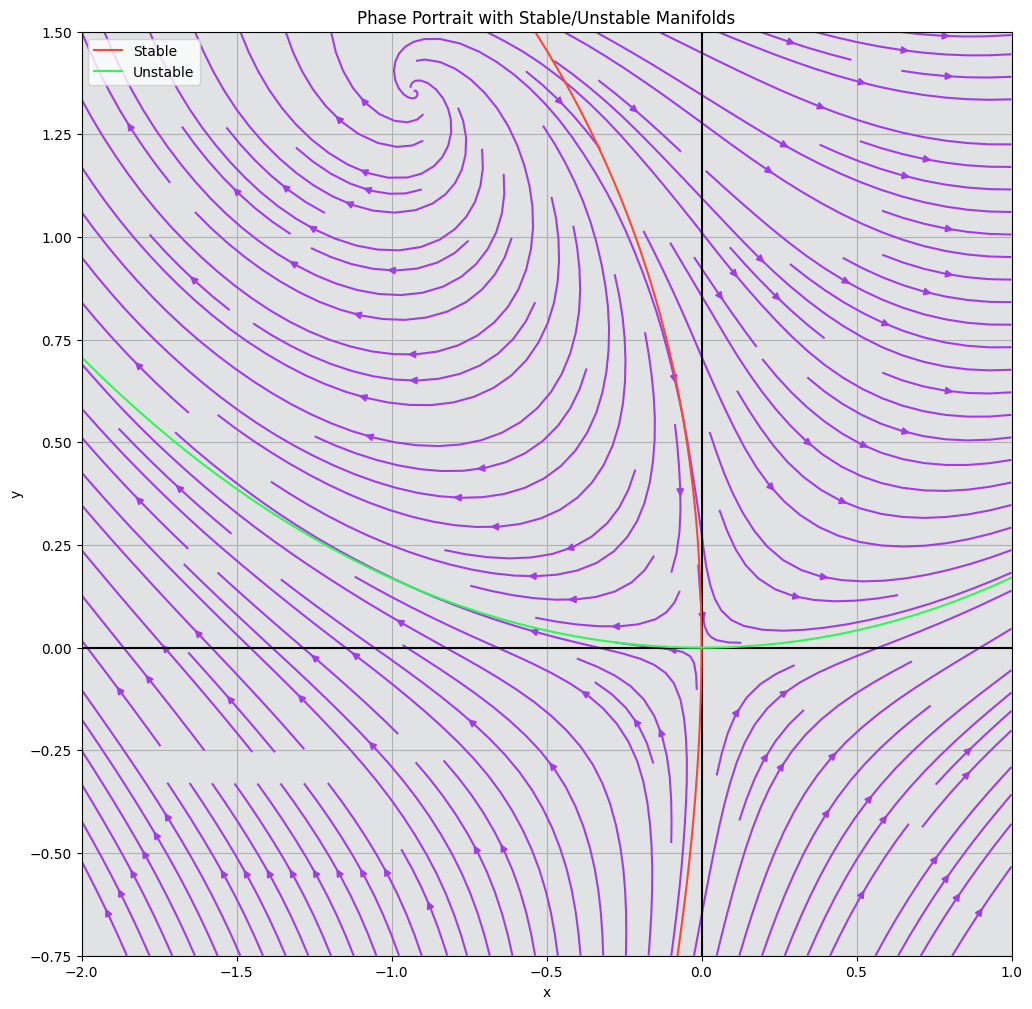
\includegraphics[width = 0.8\textwidth]{Images/Phase Portrait.png}
        \caption{Phase Portrait along with unstable and stable manifolds for the system in Problem 1.}
        \label{fig:p1a streamplot}
    \end{figure}

\clearpage
\begin{lstlisting}
import numpy as np
import matplotlib.pyplot as plt 
from scipy.integrate import solve_ivp
import matplotlib.cm as cm

def stable_manifold(y):
    return -(1/6)*y**2 -(1/24)*y**3 -(1/240)*y**4

def unstable_manifold(x):
    return (1/6)*x**2 + (1/360)*x**4 +(1/1296)*x**5 + (1/3024)*x**6

fig, axs = plt.subplots(1, 1, figsize =(12, 12))
#Vector field
xvect, yvect= np.meshgrid(np.linspace(-2, 1, 20),  
                   np.linspace(-0.75, 1.5, 10)) 

#Update vector field
u = 2*xvect + yvect**2
v = -2*yvect + xvect**2 + yvect**2

#Plotting Stream plot
axs.streamplot(xvect,yvect,u,v, density=1.4, linewidth=None, color='#A23BEC' ) 

#Plotting x any y axes
axs.plot(np.linspace(0, 0, 20), np.linspace(-0.75, 1.5, 20), color='k')
axs.plot(np.linspace(-2, 1, 20), np.linspace(0, 0, 20), color='k')
axs.grid(True)
axs.set_facecolor("#e1e2e3")
#Getting stable manifold
ypts = np.linspace(-0.75,1.5,50) 
stable = list(map(stable_manifold, ypts))

#Getting unstable manifold
xpts = np.linspace(-2,1,50) 
unstable = list(map(unstable_manifold, xpts))

#Plotting manifolds
axs.plot(stable, ypts, label = "Stable", color="#ff4534")
axs.plot(xpts, unstable, label = "Unstable", color="#2ff754")

axs.set_xlabel("x")
axs.set_ylabel("y")
plt.title("Phase Portrait with Stable/Unstable Manifolds")
axs.legend()

# Show plot with grid 
 
plt.show() 
\end{lstlisting}
\end{solution}

\newpage
\subsection{Problem 1, part b}
How might you use your local stable manifold to approximate a global one for this problem? How well does your approach work?

\end{document}